\subsubsection{Interaction between entities}

The application contains several interactions among entities that have to be
specified in order to clearly understand how to approach different problems.

\paragraph{Entering a road} Moving entities enter a road which, by accessing
one of its lane, satisfies two requirements:

\begin{itemize}
  \item the specific entity type can drive or walk on the lane. For example,
  a car can not drive on a sidewalk but only on a roadway;
  \item assuming that the moving entity wants to go in the direction $d_1$,
    then the lane has to be walkable in the direction $d_0 \rightarrow d_1$.
\end{itemize}

\paragraph{Entering a lane}
Moving entities enter a lane by simply entering its first stretch.

\paragraph{Entering a road stretch}
Moving entities who want to enter a new road stretch can do it whenever there
is room for them in that stretch.
In particular, a roadway lane stretch can be trod for at most one vehicle at a
time.

\paragraph{Zebra crossings}
Vehicles which want to enter a road stretch with painted zebra crossings have
to wait for pedestrians or bikes to free the crossing.
In our system unprivileged entities stop when a privileged entity is entering
or is already crossing the stretch they want to enter.
%TODO: Provide graphic example?

\paragraph{Crossroads} Every road that is connected to a crossroads is marked
with a cardinal point (N/E/W/S). The crossroads holds all the logic necessary
for vehicles to follow the yield rules we described in
\ref{sec:pa-app-problems}.

% verifica risposta Sebastiano
However there could be a situation in which there is a standstill,
for example when four cars simultaneously want to go straight in
a four-way crossroads each one by entering a different way of it.
In this case, the crossroads has to make a car yield the right-of-way
to another one.

Pedestrians and bikes can only walk on the corner of the crossroads, thus
passing to the adjacent piece of road.
For example, a pedestrian coming from the ``southern'' side of the
western road can only enter the southern street on the ``western'' side.

\paragraph{Entering a building}
When a moving entity is in the stretch where there is the entrance of a
building, then it can enter the building. If the entity is a pedestrian, then
it will enter the house. If the moving entity is a vehicle then it will
enter the garage. The garage has a maximum capacity and only a vehicle
which have book its parking slot can enter the garage.

\paragraph{Exiting a building}
When a moving entity is exiting a building, it has to check whether there is
room for it to move out.

\paragraph{Choosing to use a vehicle}
A person $p$ who wants to leave a building $b_1$ to move to $b_2$ can decide
to take one of the available vehicles in the garage.

When $p$ decides to get out $b_1$ with a vehicle,
all other people in $b_1$
can share the vehicle with $p$ if the logical disjunction
of the following conditions is satisfied:
\begin{itemize}
\item they share the same path;
\item they have a destination $c$ contained into $p$'s path;
\item they have a path containing $b_2$
\end{itemize}
They will leave $b_1$ with $p$ sharing a vehicle
until the most capacious vehicle, among the available ones, become full.

Nevertheless $p$ can leave $b_1$ with a vehicle only if logical disjunction
of the following conditions holds:
\begin{itemize}
\item the capacity of $b_2$'s car park is greater than the sum of all
vehicles being already there and the ones which are coming there;
\item there is at least another person in $b_1$
  \begin{itemize}
  \item having a path containing $b_2$; and
  \item ending with a building $d$, having a car park capacity that is
    greater than the sum of all vehicles being already there and the ones
    which are coming there.
  \end{itemize}
\end{itemize}
Hence, if the condition is met, the destination building books
a parking lot for the vehicle.

\begin{figure}[H]
\centering
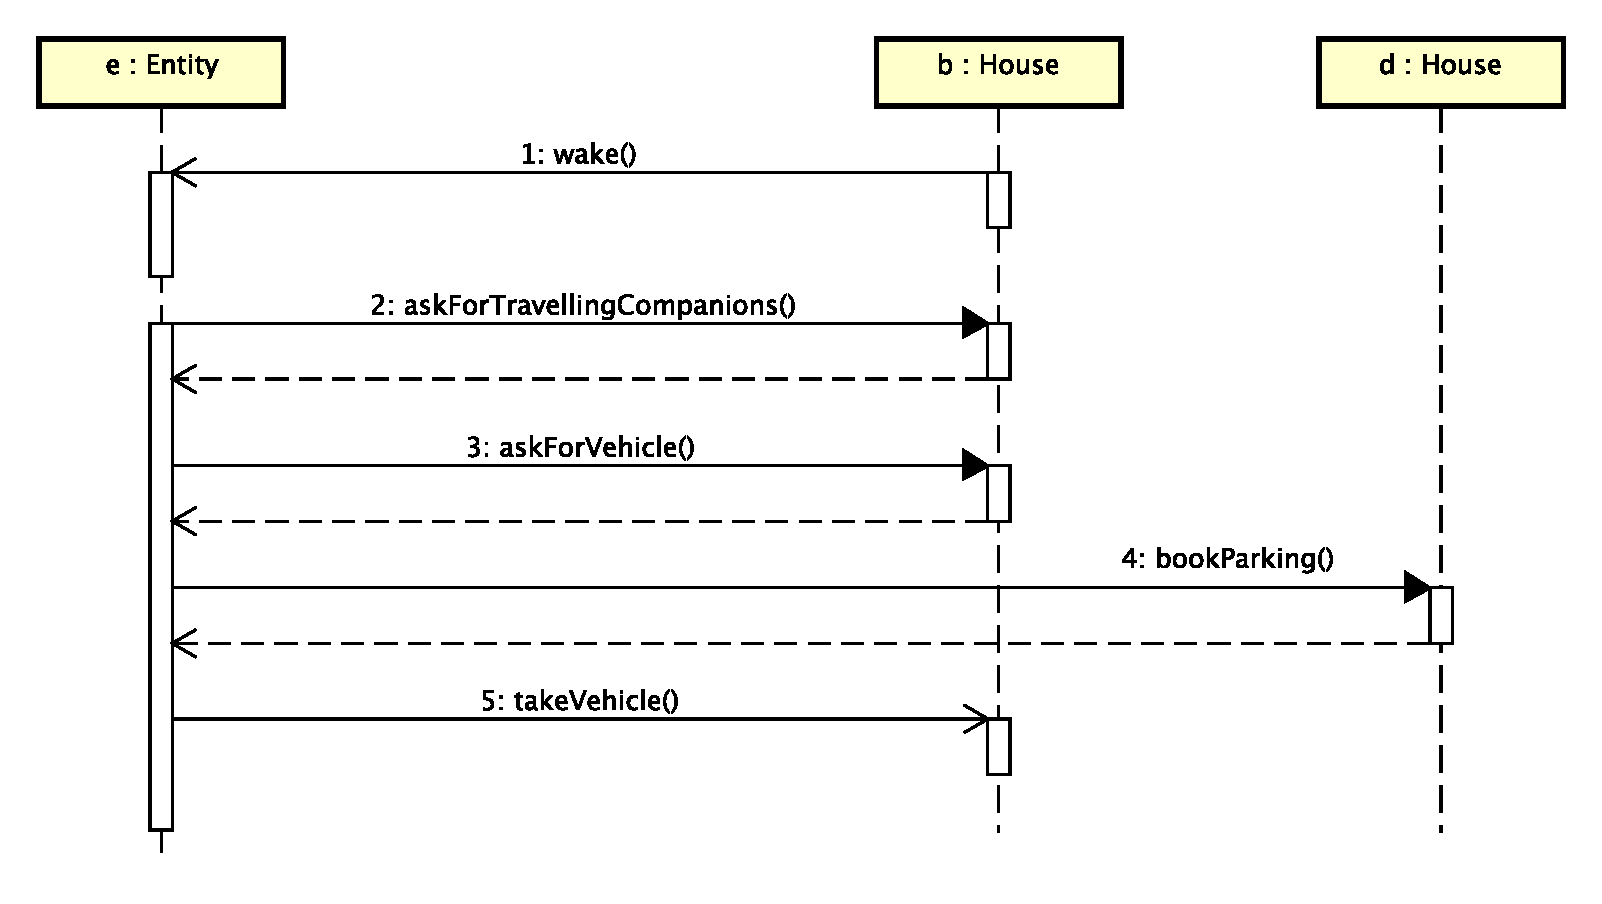
\includegraphics[width=\columnwidth,trim=1 0 0 0,clip]
  {images/solution/going_out_with_vehicle.eps}
\caption{Exiting a building with a vehicle}
\label{fig:app-inter-vehicle}
\end{figure}

\paragraph{Waiting for a bus}
Whenever a pedestrian is on a bus stop stretch, it can decide to wait for a
bus.

Firstly, the pedestrian checks whether his path is contained in the bus path.
If so, then it waits for the bus. In this case the pedestrian assumes that
the bus sooner or later will arrive.

\begin{figure}[H]
  \centering
  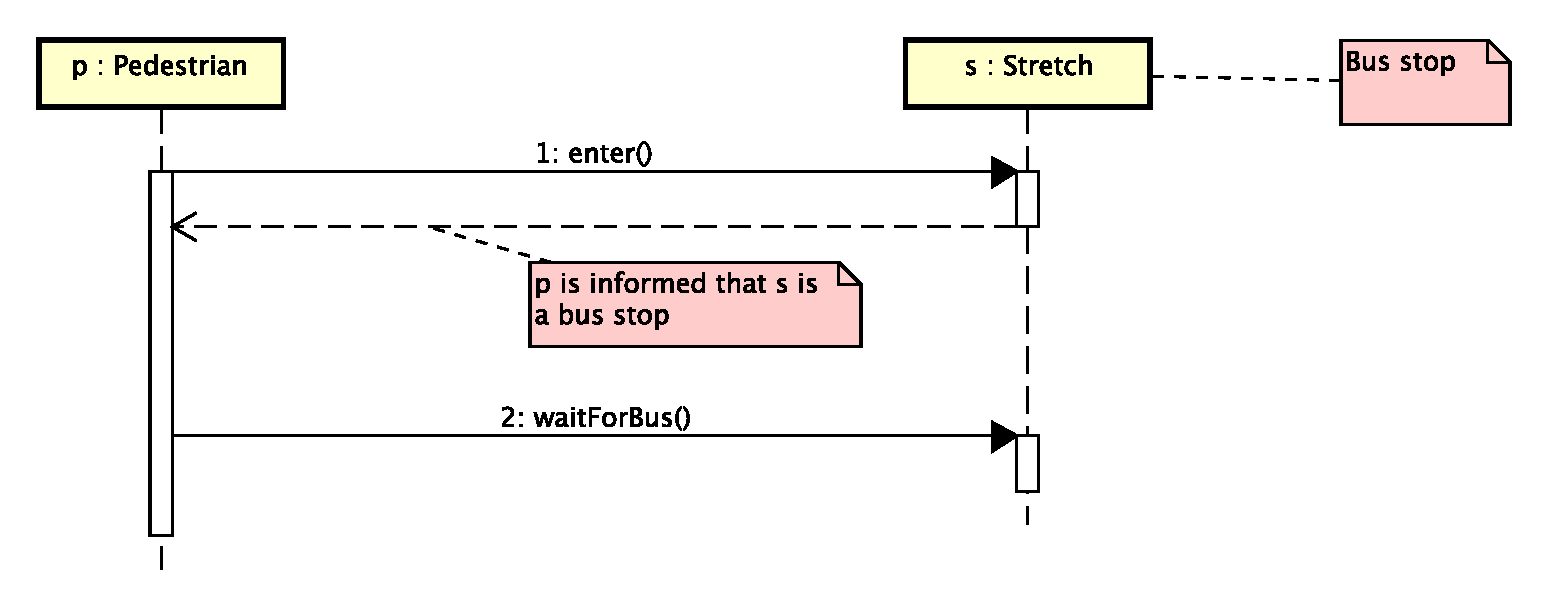
\includegraphics[width=\columnwidth,trim=1 0 2 0,clip]
    {images/solution/bus_waiting.eps}
  \caption{Waiting for a bus}
  \label{fig:app-inter-wait-bus}
\end{figure}

\paragraph{Boarding a bus}
When a bus arrives at a bus stop, then a waiting pedestrian will board it only
if there is enough room for it on the vehicle.

\begin{figure}[H]
  \centering
  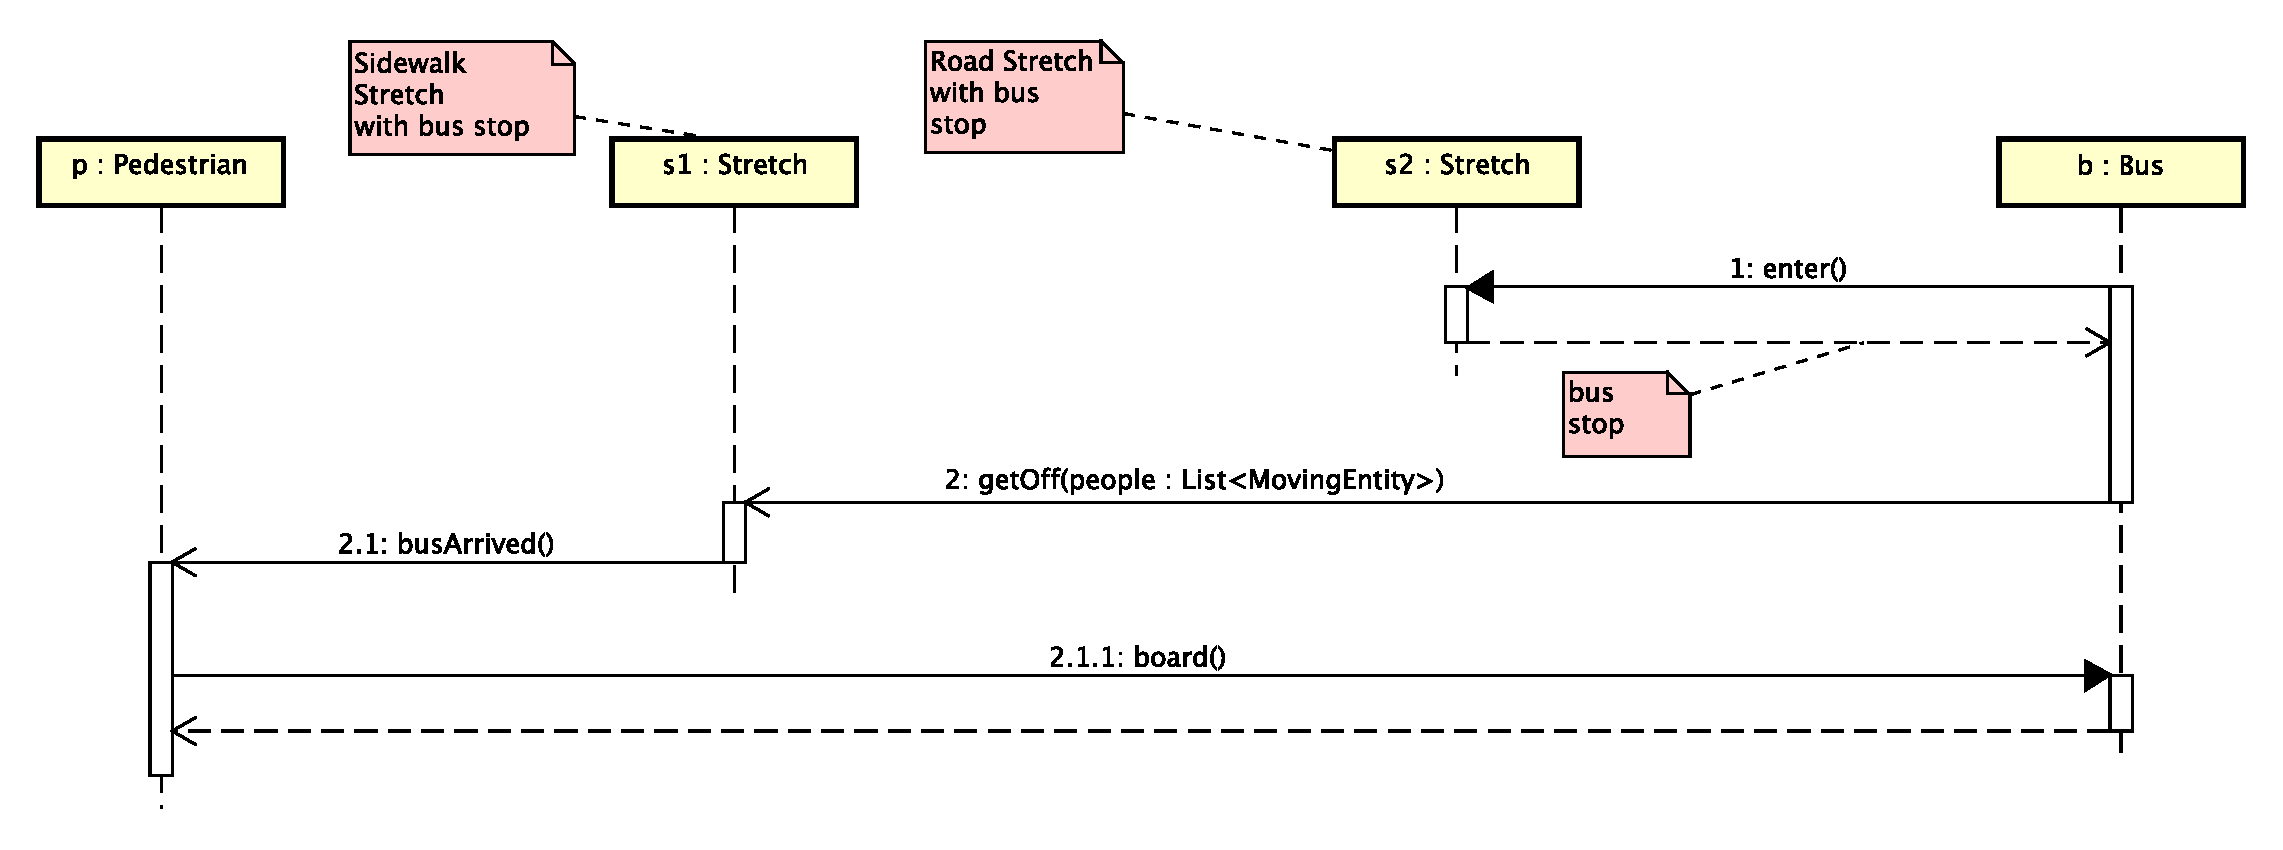
\includegraphics[width=\columnwidth,trim=1 0 0 0,clip]
    {images/solution/bus_boarding.eps}
  \caption{Boarding a bus}
  \label{fig:app-inter-board-bus}
\end{figure}

\paragraph{Getting off a bus} A person $p$ will get off a bus when it reaches
the last stop $s$ belonging to the route of $p$.

\paragraph{Respecting the road code} The roads and the crossroads contain
all the necessary logic to make moving entities respect the road rules.

\paragraph{Performing an overtaking} This action is possible only when a
vehicle is able to change lane. The vehicle performs an overtaking
only if the next stretch in its path is already taken by another moving entity.
When a vehicle tries to overtake another one, it will always try to return to
the lane where it started the operation before entering the last stretch. This
is achieved by booking the landing stretch before performing the
overtaking.

